\section{Μοντέλα CNN}
\label{sec:cnn_impl}

Όπως αναφέραμε \autoref{sec:dnn_sw}, το βασικό εργαλείο λογισμικού που
χρησιμοποιήσαμε για την ανάπτυξη των μοντέλων CNN είναι το \emph{Keras}.

Η βιβλιοθήκη Keras προσφέρει τις υλοποιήσεις όλων των επιπέδων που
απαιτούνται για για την ανάπτυξη ενός CNN
\footnote{Πλήρες περιγραφή της λίστας των διαθέσιμων επιπέδων: \href{https://keras.io/layers/core/}{https://keras.io/layers/core/}}.
Πιο συγκεκριμένα, τα επίπεδα που χρησιμοποιήθηκαν, καθώς και οι βασικές
παράμετροι τους περιγράφονται πιο κάτω:
\begin{itemize} % Below why the first bold and the other not?
  \item{\textbf{InputLayer}: Επίπεδο Εισόδου του νευρωνικού δικτύου}
    \begin{itemize}
      \item{Διαστάσεις του όγκου εισόδου (tensor shape)}
    \end{itemize}
  \item{Convolution2D: Επίπεδο Συνέλιξης}
    \begin{itemize}
      \item{Μορφολογία της εισόδου}
      \item{Αριθμός των φίλτρων συνέλιξης}
      \item{Διαστάσεις των φίλτρων συνέλιξης}
      \item{Συνάρτηση ενεργοποίησης}
    \end{itemize}
  \item{MaxPooing2D: Επίπεδο Υποδειγματοληψίας}
    \begin{itemize}
      \item{Διαστάσεις πλαισίου}
      \item{Βήμα μετατόπισης}
    \end{itemize}
  \item{ZeroPadding2D: Προσθέτει πλαίσιο με μηδενικά στον όγκο εισόδου}
    \begin{itemize}
      \item{Διαστάσεις του πλαισίου}
    \end{itemize}
  \item{Activation: Επίπεδο ενεργοποίησης. Εφαρμόζει συνάρτηση ενεργοποίησης στον
    όγκο εξόδου του προηγούμενου επιπέδου}
  \item{Dropout: Επίπεδο πρόληψης υπέρ-προσαρμογής \cite{lecun2015deep}}
  \item{Dense: Πλήρες συνδεδεμένο επίπεδο}
    \begin{itemize}
      \item{Διαστάσεις του όγκου εισόδου (Προαιρετικό)}
      \item{Διαστάσεις του όγκου εξόδου}
      \item{Συνάρτηση ενεργοποίησης}
    \end{itemize}
  \item{Flatten: Μετασχηματίζει τον όγκου εισόδου σε επίπεδη αναπαράσταση
    (π.χ. για όγκο εισόδου $64 \times 32 \times 32$ η έξοδος θα είναι επίπεδη με $65536$ νευρώνες)}
  \item{BatchNormalization: Εφαρμόζει μετασχηματισμό για να διατηρήσει την μέση τιμή
      και την τυπική απόκλιση των ενεργοποιήσεων του προηγούμενου επιπέδου στις τιμές 0 και 1 αντίστοιχα}
\end{itemize}

Σημαντική παρατήρηση είναι το γεγονός ότι η επιστήμη της βαθιάς μηχανικής μάθησης
βρίσκεται σε πρώιμο στάδιο, με αποτέλεσμα να μην υπάρχουν συγκεντρωμένες
οι υλοποιήσεις των διαφόρων επιπέδων και γενικότερα των μοντέλων σύγχρονων ΑNN.

Περαιτέρω, η επιλογή των μοντέλων CNN στηρίχθηκε στην ύπαρξη
προ-εκπαιδευμένων βαρών για τα αντίστοιχα CNN στο διαδίκτυο για 2 λόγους:
\begin{itemize}
  \item{Η διαδικασία εκπαίδευσης είναι χρονοβόρα διαδικασία και προϋποθέτει
    τη χρήση μίας ή περισσοτέρων ισχυρών μονάδων GPU (NVIDIA Titam X GPU)}
  \item{Η εκπαίδευση νευρωνικών δικτύων ξεφεύγει από τα πλαίσια της παρούσας
    διπλωματικής εργασίας}
\end{itemize}


\subsection{AlexNet}

Το δίκτυο AlexNet ήταν η αρχή της εισαγωγής της βαθιάς
μηχανικής μάθησης στην επιστήμη της μηχανικής όρασης. Εμφανίστηκε και χρησιμοποιήθηκε
στον διαγωνισμό ImageNet ILSVRC challenge, το 2012, κερδίζοντας με διαφορά
10,9\%, στο σφάλμα αναγνώρισης αντικειμένων σε σύνολο 1000 κλάσεων.

\begin{figure}[!ht]
  \centering
  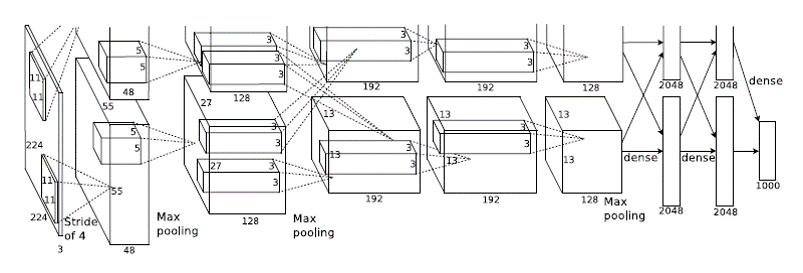
\includegraphics[width=1\textwidth]{./images/chapter5/alexnet_from_paper.png}
  \caption[Μοντέλο δικτύου AlexNet]{%
    Μοντέλο δικτύου AlexNet \cite{NIPS2012_4824}
  }
  \label{fig:alexnet_from_paper}
\end{figure}

Το συγκεκριμένο νευρωνικό δίκτυο συνέλιξης αποτελείται από σύνολο οκτώ επίπεδα,
ή καλύτερα ομάδες επιπέδων; πέντε (5) επίπεδα συνέλιξης και τρία (3) πλήρως συνδεδεμένα. \\

\begin{tabular}{ | l | l | l | l | }
  \hline
  \rowcolor{Gray}
  Επίπεδο  & Τύπος & Αριθμός καναλιών & Διαστάσεις φίλτρων \\
  \hline
  1 & Conv+Pool+Norm & 96 & $11 \times 11$ \\
  2 & Conv+Pool+Norm & 256 & $5 \times 5$ \\
  3 & Conv & 384 & $3 \times 3$ \\
  4 & Conv & 384 & $3 \times 3$ \\
  5 & Conv+Pool & 256 & $3 \times 3$ \\
  6 & Full & 4096 & Ν/A \\
  7 & Full & 4096 & N/A \\
  8 & Full & 1000 & N/A \\
  \hline
\end{tabular}
\\

Η συνάρτηση υποδειγματοληψίας που χρησιμοποιεί το μοντέλο είναι η συνάρτηση
MaxPooling2D με βήμα μετατόπισης ίσο με την μονάδα και στους 2 άξονες ($1 \times 1$).
Σε όλα τα επίπεδα εκτός του τελευταίου χρησιμοποιήθηκε η συνάρτηση ενεργοποίησης
ReLU. Επίσης χρησιμοποιεί και πολλά επίπεδα ZeroPadding με πλαίσιο
διαστάσεων $1 \times 1$. Το τελευταίο επίπεδο παίζει τον ρόλο του ταξινομητή και συγκεκριμένα
είναι ένας ταξινομητής Softmax.

Η υλοποίηση στηρίχτηκε στην αντίστοιχη που υπάρχει με το εργαλείο Caffe
\footnote{Υλοποίηση του δικτύου AlexNet στο Caffe: \url{https://github.com/BVLC/caffe/tree/master/models/bvlc_alexnet}}.
Πρακτικά μεταφράστηκε ο πηγαίος κώδικας της υλοποίησης από το Caffe στο Keras.
Ο αντίστοιχος γράφος της υλοποίησης του μοντέλου
φαίνεται φαίνεται στο \autoref{fig:alexnet_2}.

\begin{figure}[!ht]
  \centering
  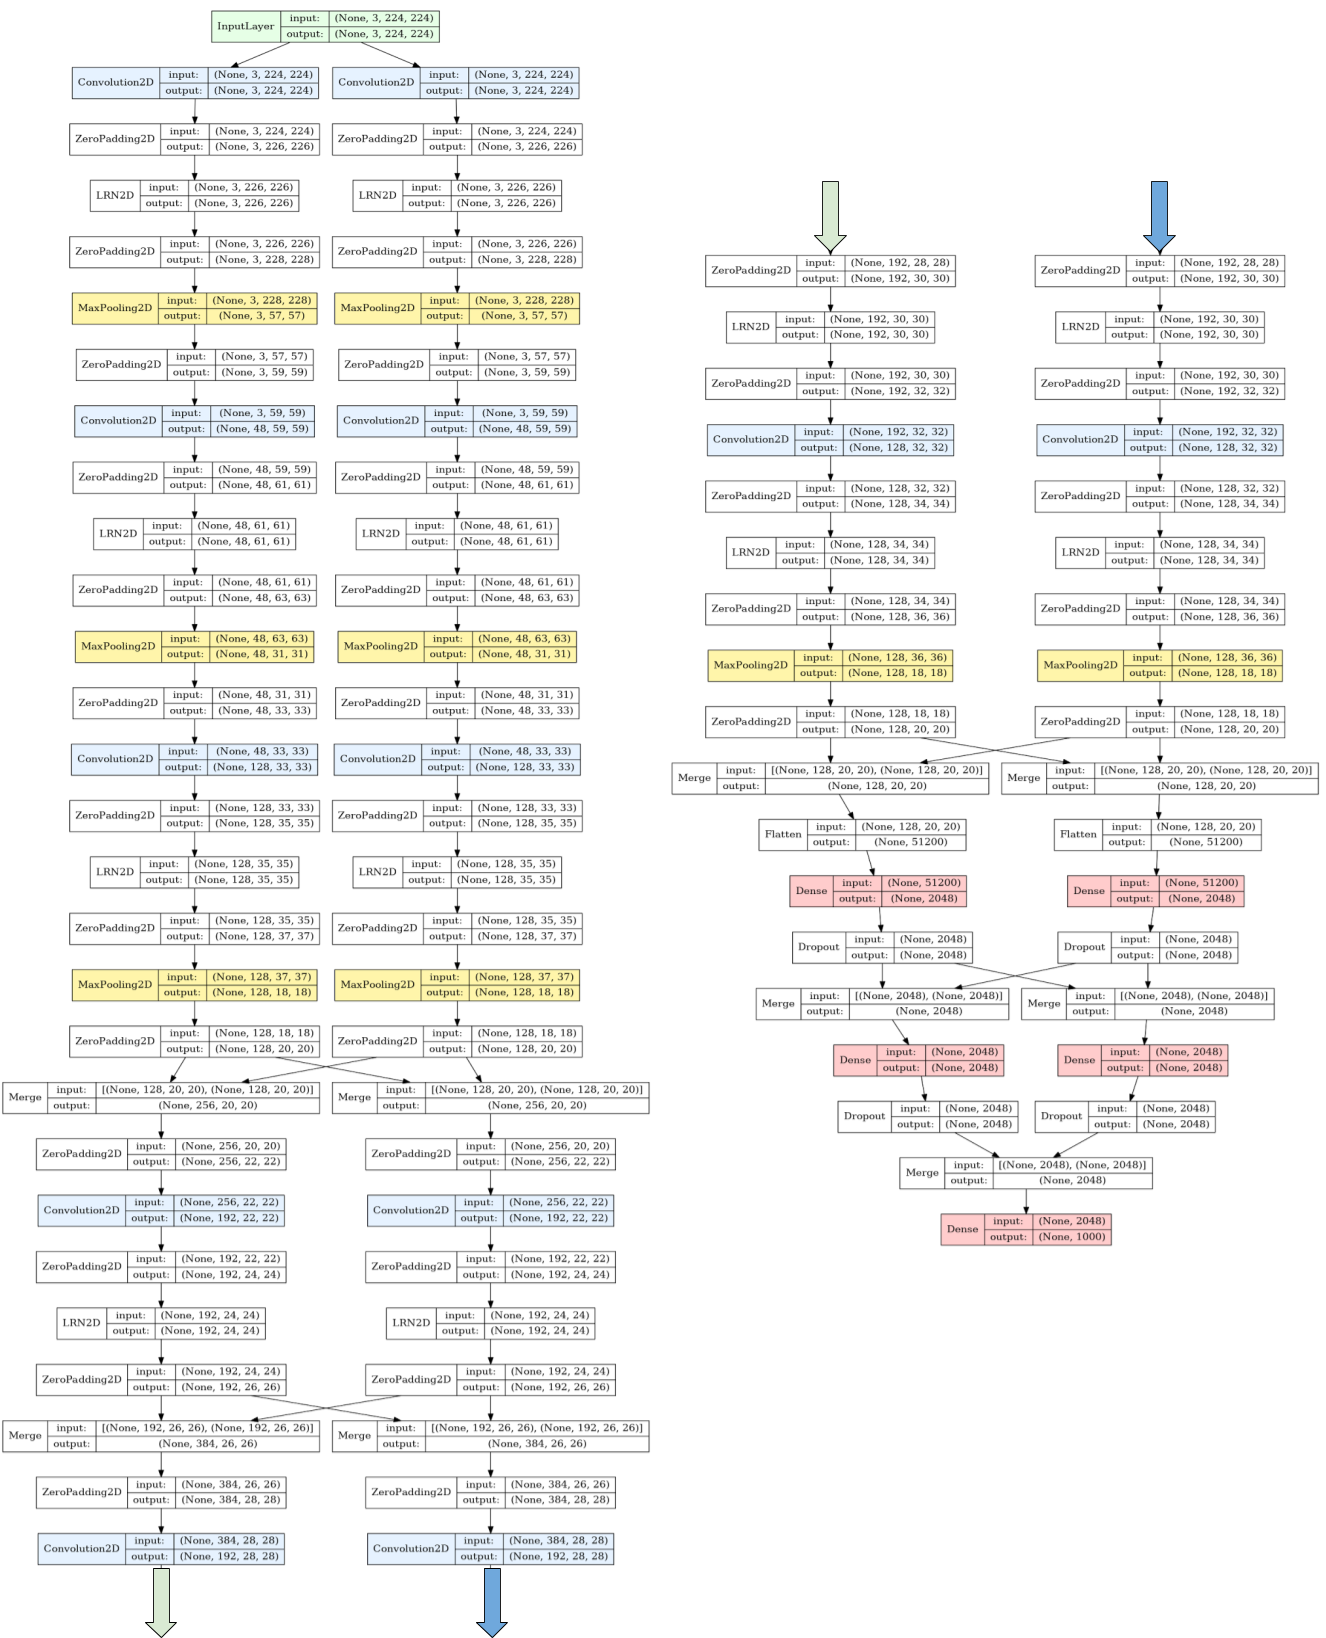
\includegraphics[width=1\textwidth]{./images/chapter5/alexnet_3.png}
  \caption[Πλήρης μορφή του δικτύου AlexNet της υλοποίησης]{Πλήρης μορφή του δικτύου AlexNet της υλοποίησης}
  \label{fig:alexnet_2}
\end{figure}

Το AlexNet είναι ένα μοντέλο που υποστηρίζει μόνο αναγνώριση και όχι εντοπισμό
των αντικειμένων, δηλαδή η μόνη πληροφορία που μας δίνει είναι η ύπαρξη των κλάσεων των
αντικειμένων.

%% --------------------------------------------------------------------------
\subsection{VGG16}

Το δίκτυο VGG16 ήταν ο νικητής του διαγωνισμού ImageNet ILSVRC-2014 με σφάλμα
κατηγοριοποίησης 7.5\% σε σύνολο 1000 κλάσεων αντικειμένων \cite{Simonyan14c}.

\begin{figure}[!ht]
  \centering
  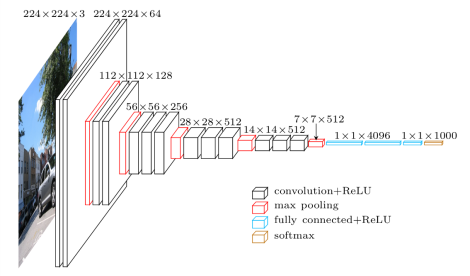
\includegraphics[width=0.8\textwidth]{./images/chapter5/vgg16_from_paper.png}
  \caption[Mορφή του δικτύου VGG16]{Μορφή του δικτύου VGG16}
  \label{fig:vgg16_from_paper}
\end{figure}

Αποτελείται από 16 επίπεδα; 13 επίπεδα συνέλιξης και 3 πλήρως συνδεδεμένα (\autoref{fig:vgg16_from_paper}), των
οποίων τα χαρακτηριστικά δίνονται πιο κάτω:
\\

\begin{tabular}{ | l | l | l | l | }
  \hline
  \rowcolor{Gray}
  Επίπεδο  & Τύπος & Αριθμός καναλιών & Διαστάσεις φίλτρων \\
  \hline
  1 & Conv & 64 & $3 \times 3$ \\
  2 & Conv+Pool & 64 & $3 \times 3$ \\
  3 & Conv & 128 & $3 \times 3$ \\
  4 & Conv+Pool & 128 & $3 \times 3$ \\
  5 & Conv & 256 & $3 \times 3$ \\
  6 & Conv & 256 & $3 \times 3$ \\
  7 & Conv+Pool & 256 & $3 \times 3$ \\
  8 & Conv & 512 & $3 \times 3$ \\
  9 & Conv & 512 & $3 \times 3$ \\
  10 & Conv+Pool & 512 & $3 \times 3$ \\
  11 & Conv & 512 & $3 \times 3$ \\
  12 & Conv & 512 & $3 \times 3$ \\
  13 & Conv+Pool & 512 & $3 \times 3$ \\
  14 & FullyConnected & 4096 & Ν/A \\
  15 & FullyConnected & 4096 & N/A \\
  16 & FullyConnected & 1000 & N/A \\
  \hline
\end{tabular}
\\

Παρομοίως με το δίκτυο AlexNet, σε όλα τα επίπεδα εκτός του τελευταίου χρησιμοποιήθηκε η συνάρτηση ενεργοποίησης
ReLU, ενώ το τελευταίο επίπεδο παίζει τον ρόλο του ταξινομητή και συγκεκριμένα
είναι ένας ταξινομητής Softmax. Το βήμα μετατόπισης των συναρτήσεων υποδειγματοληψίας
είναι διαστάσεων $1 \times 1$.

Το μοντέλο του δικτύου VGG16 υπάρχει υλοποιημένο στην λίστα με τα παραδείγματα
του εργαλείου Keras \footnote{\url{https://github.com/fchollet/keras/tree/master/keras/applications}}.
Ο αντίστοιχος γράφος της υλοποίησης του μοντέλου
φαίνεται στο \autoref{fig:vgg16}.

\begin{figure}[!ht]
  \centering
  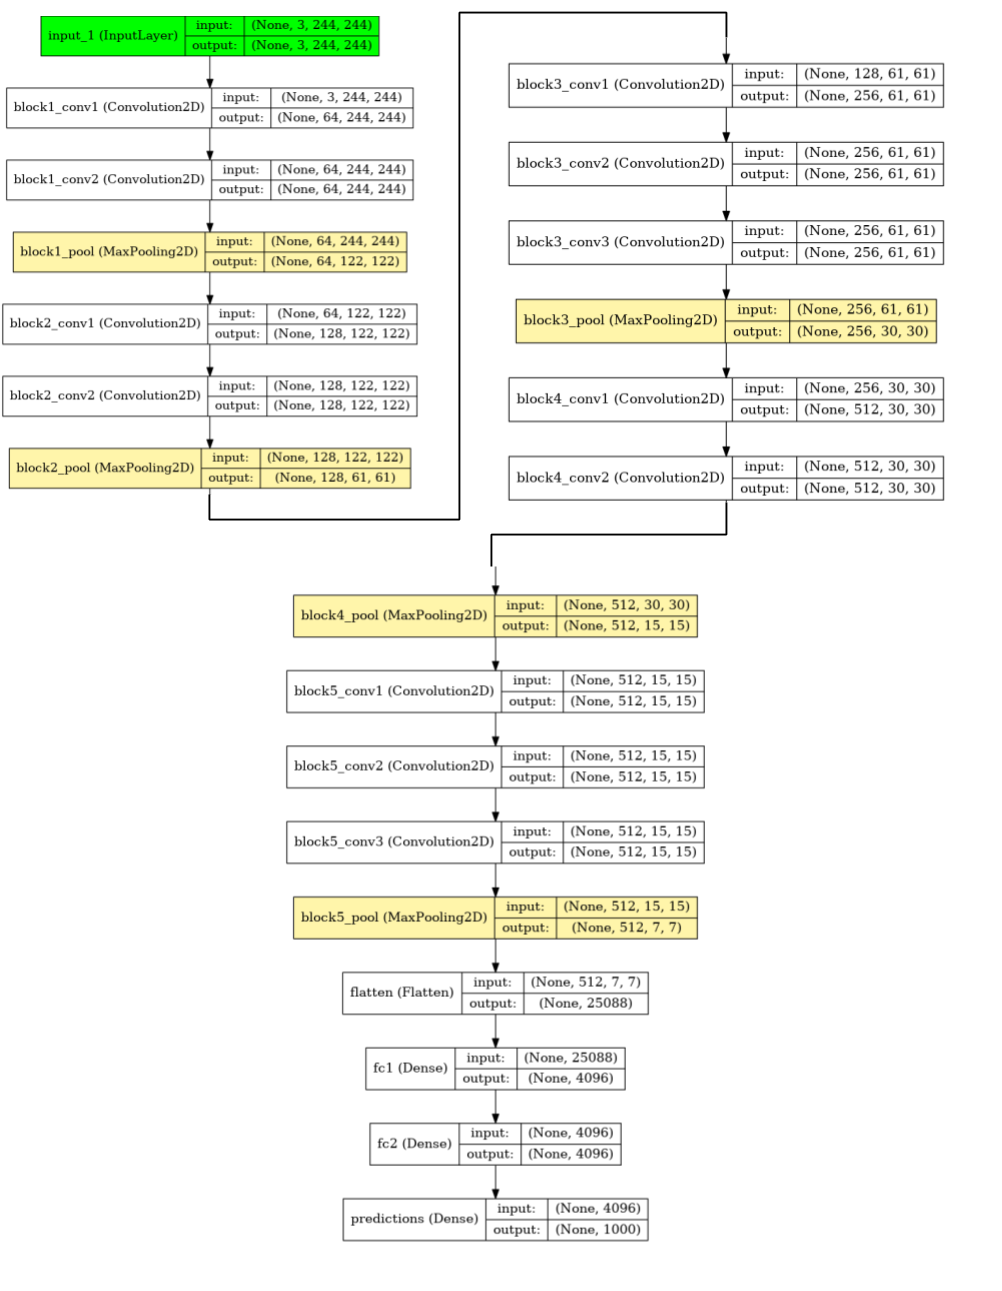
\includegraphics[width=0.9\textwidth]{./images/chapter5/vgg16.png}
  \caption[Πλήρης μορφή του δικτύου VGG16 της υλοποίησης]{Πλήρης μορφή του δικτύου VGG16 της υλοποίησης}
  \label{fig:vgg16}
\end{figure}

%% --------------------------------------------------------------------------
%\subsection{GoogleNet aka Inception-V1}

%\textbf{Να το προσθέσουμε και αυτό?}

%% --------------------------------------------------------------------------
\subsection{YOLO Net}

Το δίκτυο YOLO (You Only Look Once), είναι το πρώτο μοντέλο νευρωνικού δικτύου
συνέλιξης το οποίο προσπαθεί να επιλύσει το πρόβλημα της ταυτόχρονης αναγνώρισης
και εντοπισμού αντικειμένων σε εικόνες, με ένα προς-τα-εμπρός πέρασμα (forward pass).
Η ιδιαιτερότητά του είναι ότι αντιμετωπίζει το πρόβλημα σαν ένα πρόβλημα
regression και όχι classification.

Μία ακόμη ιδιαιτερότητα του συγκεκριμένου δικτύου είναι ότι θέτει σαν απαίτηση
την εφαρμογή του σε προβλήματα σχεδόν πραγματικού χρόνου και άρα στοχεύει κυρίως
στην ταχύτητα της αναγνώρισης. Φυσικά αυτό έχει σαν αποτέλεσμα την μείωση της ακρίβειας
αναγνώρισης, η οποία είναι χαμηλότερη σε σχέση με άλλα μοντέλα, όπως για παράδειγμα τα δίκτυα
Fast-RCNN \cite{DBLP:journals/corr/Girshick15}, Overfeat και DetectorNet.

Η έξοδος του δικτύου αντιστοιχεί τόσο στις κλάσεις των αντικειμένων
που αναγνωρίστηκαν, καθώς και στις συντεταγμένες όπου αυτά εντοπίστηκαν.

\begin{figure}[!ht]
  \centering
  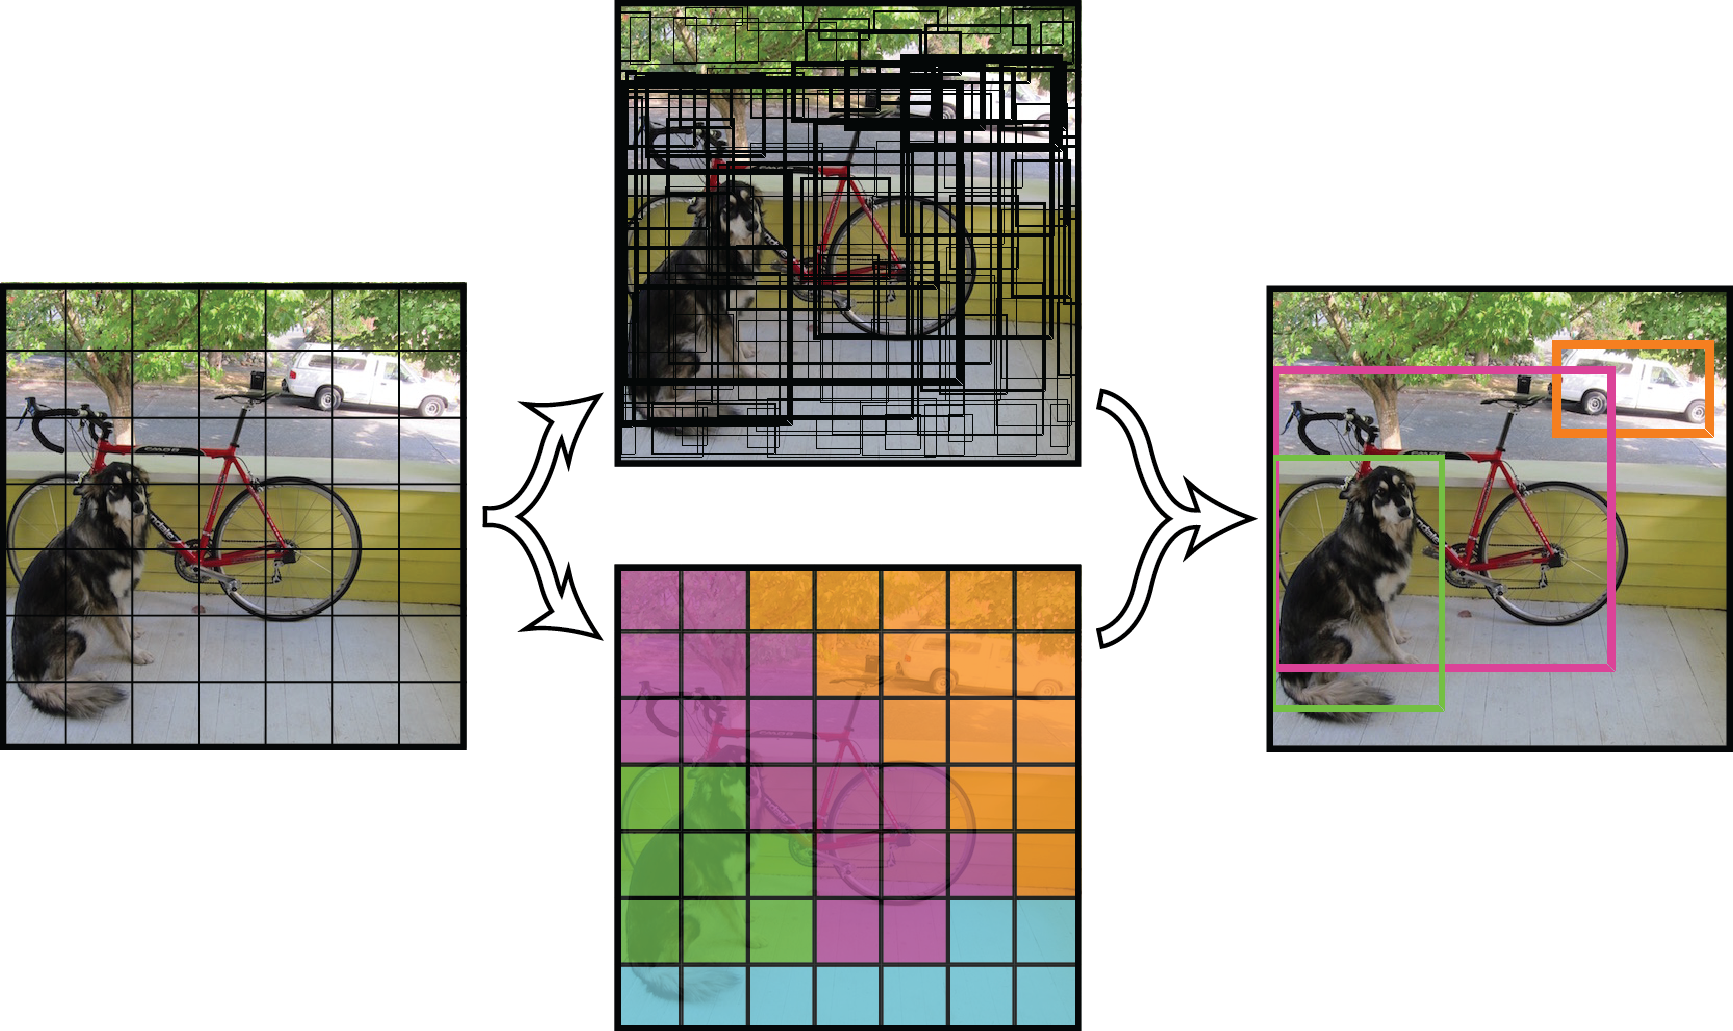
\includegraphics[width=0.8\textwidth]{./images/chapter5/yolonet_from_paper_1.png}
  \caption[Παράδειγμα τρόπου λειτουργίας του δικτύου YOLO]{Παράδειγμα τρόπου λειτουργίας του δικτύου YOLO}
  \label{fig:yolonet_from_paper}
\end{figure}

Το βασικό μοντέλο του δικτύου YOLO έχει την δυνατότητα να επεξεργάζεται εικόνες με ταχύτητα
\emph{45 fps} χρησιμοποιώντας μονάδα GPU (Nvidia Titan X).

Λόγω της ιδιαιτερότητας του συγκεκριμένου δικτύου, όσον αφορά τον τρόπο προσέγγισης του προβλήματος της ταυτόχρονης
αναγνώρισης και εντοπισμού των αντικειμένων, θεωρούμε σημαντικό να αναφέρουμε
και να εξηγήσουμε τον τρόπο λειτουργίας του.
Το πρώτο βήμα είναι να χωρίσει την εικόνα εισόδου σε ένα πλέγμα διαστάσεων $S \times S$
(αριστερή εικόνα στο \autoref{fig:yolonet_from_paper}).
Κάθε κελί του πλέγματος προβλέπει $B$ οριοθετημένα πλαίσια (bounding boxes) μαζί με ένα σκορ
"εμπιστοσύνης" για το κάθε πλαίσιο (πάνω μεσαία εικόνα στο \autoref{fig:yolonet_from_paper}).
Το σκορ εμπιστοσύνης ερμηνεύεται ως η βεβαιότητα
να ανήκει ένα αντικείμενο στο συγκεκριμένο πλαίσιο μαζί με την ακρίβεια ότι
το συγκεκριμένο αντικείμενο ανήκει σε αυτό το πλαίσιο. Η μαθηματική έκφραση
ορίζεται ως:
\begin{equation*}
  confidence = P(object | box = \imath) * IOU_{pred}^{truth}
\end{equation*}
Από την παραπάνω μαθηματική έκφραση καταλαβαίνουμε ότι σε περίπτωση που
σε ένα κελί δεν υπάρχει αντικείμενο, το σκορ εμπιστοσύνης μηδενίζεται.
Επίσης, κάθε κελί του πλέγματος προβλέπει και τις πιθανότητες της κλάσης
του αντικειμένου, $P(class_{\imath} | object)$
(κάτω μεσαία εικόνα στο \autoref{fig:yolonet_from_paper}).

Χρησιμοποιώντας τις 2 αυτές μαθηματικές εκφράσεις των υπό-συνθήκη πιθανοτήτων,
καταλήγουμε στην σχέση
\begin{equation*}
  \begin{aligned}
    class-confidence = {} & P(class_{\imath} | object) * P(object | box = \imath) * IOU_{pred}^{truth} = \\
                          & P(class_{\imath}) * IOU_{pred}^{truth}
  \end{aligned}
\end{equation*}
η οποία μας δίνει το σκορ εμπιστοσύνης για μία συγκεκριμένη κλάση.

Κάθε οριοθετημένο πλαίσιο αποτελείται από πέντε προβλέψεις; $x, y, w, h$ και
το σκορ εμπιστοσύνης. Τα $x$ και $y$ αντιστοιχούν στις συντεταγμένες του
κέντρου του πλαισίου ενώ οι τιμές των $w$ και $h$ αναφέρονται στο
μήκος και το πλάτος του.

Τέλος, οι προβλέψεις στην έξοδο του δικτύου φαίνονται σαν ένας όγκος
διαστάσεων
\begin{equation*}
  S \times S \times (B * 5 + C)
\end{equation*}

Το πλήρες μοντέλο YOLO αποτελείται από 24 επίπεδα συνέλιξης και 2 πλήρως
συνδεδεμένα.

Πέρα από το πλήρες μοντέλο, έχει σχεδιαστεί και εκπαιδευτεί, από την ίδια ομάδα ερευνητών, ένα μοντέλο
με παρόμοιο τρόπο λειτουργίας αλλά με πολύ λιγότερα επίπεδα συνέλιξης και άρα πιο
γρήγορο στην εκτέλεση (Tiny/Fast YOLO). Το TinyYOLO αποτελείται από 9 επίπεδα
συνέλιξης και 2 πλήρως συνδεδεμένα. Σε όλα τα επίπεδα εκτός του τελευταίου
χρησιμοποιείται η συνάρτηση ενεργοποίησης LeakyReLU που παρουσιάστηκε στο \autoref{sec:theory_cnn}.

Η υλοποίηση μας στηρίχτηκε στην αντίστοιχη του μοντέλου Tiny-YOLO που έγινε από
την αντίστοιχη ερευνητική ομάδα \footnote{Βασική υλοποίηση του δικτύου YOLO: \url{http://pjreddie.com/darknet/}}
\cite{darknet13}.

Θεωρούμε σημαντικό να αναφέρουμε ότι αρχικά προσπαθήσαμε να τρέξουμε την βασική υλοποίηση,
η οποία είναι γραμμένη σε γλώσσα προγραμματισμού \emph{C}, ανεπιτυχώς.
Η εκτέλεση του προγράμματος υλοποίησης του μοντέλου Tiny-YOLO εμφανίζει σφάλματα
τύπου \emph{segmentation fault}.
